\section{Horse Owner}

\subsection{Login}

\textbf{Role:} Horse Owner

\begin{itemize}
    \item \textbf{Function trigger:} The owner enters account credentials to log in.

    \item \textbf{Function description:}
    \begin{itemize}
        \item \textbf{Purpose:}
        \begin{enumerate}
            \item Verify the owner's identity.
            \item Grant access to owner functionalities.
        \end{enumerate}

        \item \textbf{Data processing:}
        \begin{enumerate}
            \item The owner enters username and password.
            \item The system validates credentials.
            \item The system identifies the OWNER role.
            \item The system creates a login session.
        \end{enumerate}
    \end{itemize}

    \item \textbf{Function details:}
    \begin{itemize}
        \item Successful login redirects to Owner Dashboard.
        \item Invalid credentials display an error message.
        \item Users without accounts may register.
    \end{itemize}
\end{itemize}

\textbf{Screen layout:}

\begin{figure}[H]
    \centering
    
\includegraphics[width=0.7\textwidth]{figures/web_application/owner/login.png}
    \caption{Horse Owner Login}
\end{figure}


\subsection{Manage Horses}

\textbf{Role:} Horse Owner

\begin{itemize}
    \item \textbf{Function trigger:} Select ``Quan ly Ngua''.

    \item \textbf{Function description:}
    \begin{itemize}
        \item \textbf{Purpose:}
        \begin{enumerate}
            \item Register new horses.
            \item Manage owned horses.
        \end{enumerate}

        \item \textbf{Data processing:}
        \begin{enumerate}
            \item Enter horse name.
            \item Enter age.
            \item Select breed.
            \item Select gender.
            \item Save horse information.
        \end{enumerate}
    \end{itemize}

    \item \textbf{Function details:}
    \begin{itemize}
        \item Add new horses.
        \item Edit horse information.
        \item Delete horse information.
        \item Display horse list.
    \end{itemize}
\end{itemize}

\textbf{Screen layout:}

\begin{figure}[H]
    \centering
    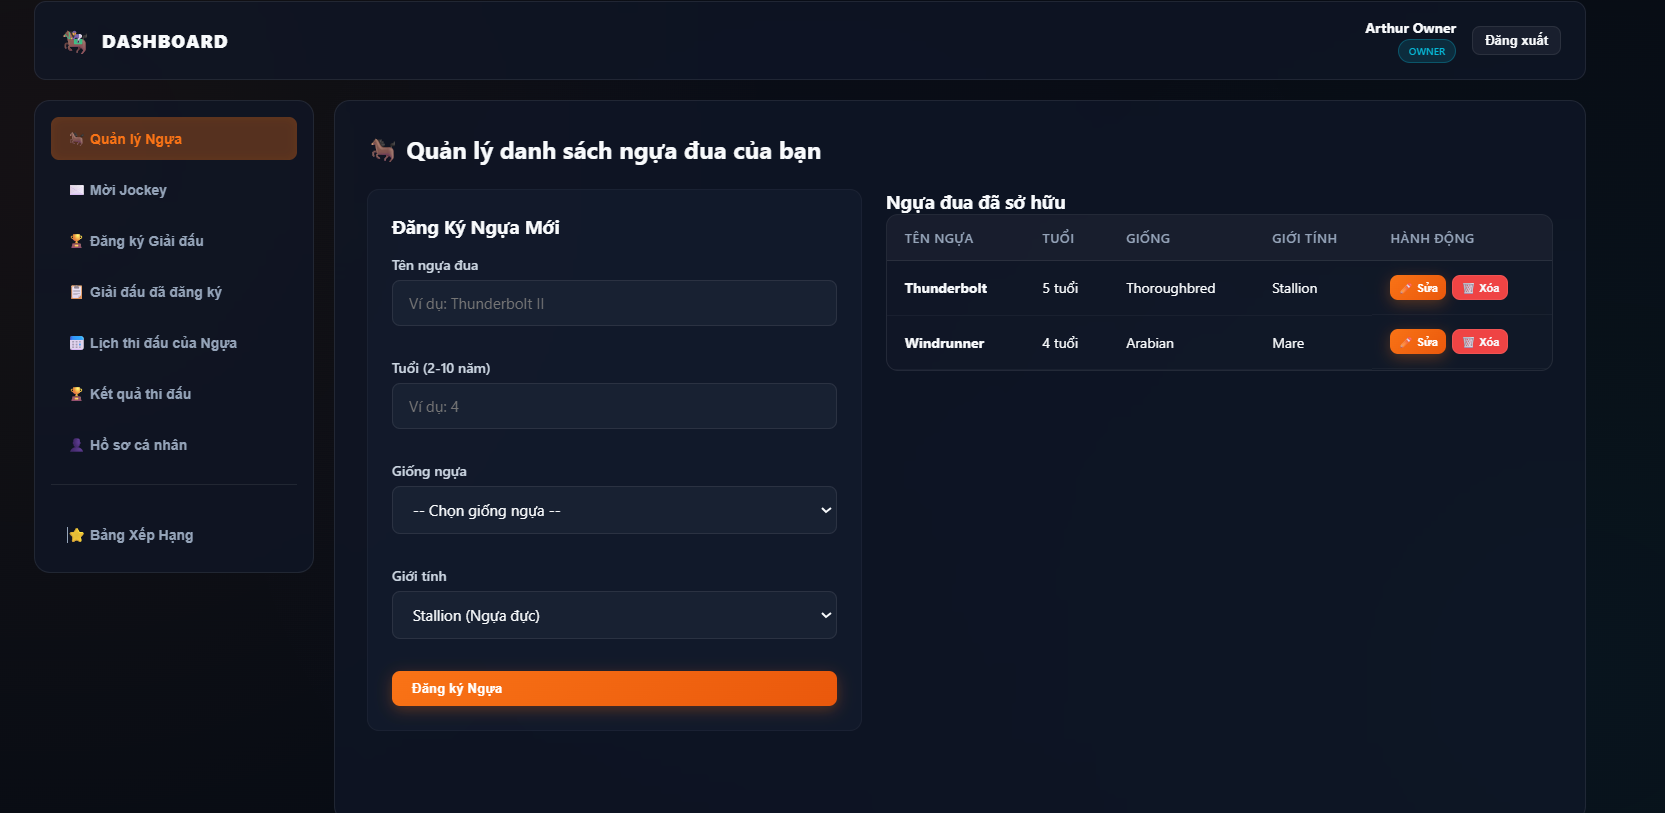
\includegraphics[width=\textwidth]{figures/web_application/owner/manage_horse.png}
    \caption{Manage Horses}
\end{figure}

% ===================================================

\subsection{Invite Jockey}

\textbf{Role:} Horse Owner

\begin{itemize}
    \item \textbf{Function trigger:} Select ``Moi Jockey''.

    \item \textbf{Function description:}
    \begin{itemize}
        \item \textbf{Purpose:}
        \begin{enumerate}
            \item Invite jockeys.
            \item Create horse-jockey partnerships.
        \end{enumerate}

        \item \textbf{Data processing:}
        \begin{enumerate}
            \item Select jockey.
            \item Select horse.
            \item Select tournament.
            \item Enter invitation message.
            \item Send invitation.
        \end{enumerate}
    \end{itemize}

    \item \textbf{Function details:}
    \begin{itemize}
        \item Invitation status is displayed.
        \item Pending invitations can be monitored.
        \item Accepted invitations may be used for registration.
    \end{itemize}
\end{itemize}

\textbf{Screen layout:}

\begin{figure}[H]
    \centering
    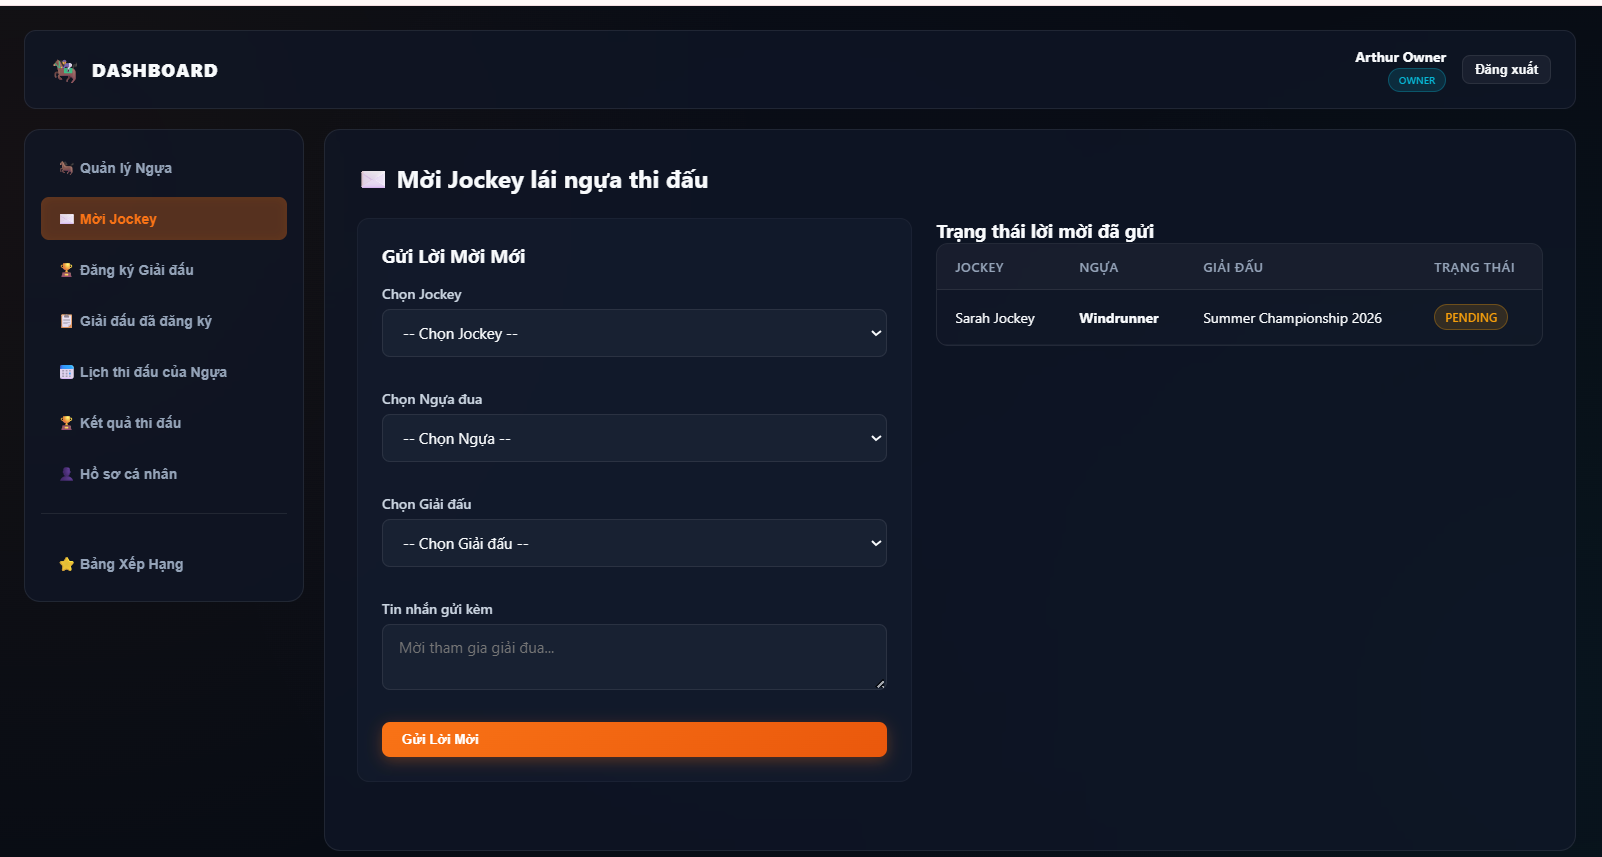
\includegraphics[width=\textwidth]{figures/web_application/owner/invite_jockey.png}
    \caption{Invite Jockey}
\end{figure}

% ===================================================

\subsection{Register Tournament}

\textbf{Role:} Horse Owner

\begin{itemize}
    \item \textbf{Function trigger:} Select ``Dang ky Giai dau''.

    \item \textbf{Function description:}
    \begin{itemize}
        \item \textbf{Purpose:}
        \begin{enumerate}
            \item Register horse-jockey pairs.
            \item Participate in tournaments.
        \end{enumerate}

        \item \textbf{Data processing:}
        \begin{enumerate}
            \item Retrieve available tournaments.
            \item Check accepted jockey invitations.
            \item Select horse-jockey pair.
            \item Submit registration request.
        \end{enumerate}
    \end{itemize}

    \item \textbf{Function details:}
    \begin{itemize}
        \item Only accepted invitations may register.
        \item Registration requests are sent to administrators.
        \item Invalid pairs cannot participate.
    \end{itemize}
\end{itemize}

\textbf{Screen layout:}

\begin{figure}[H]
    \centering
    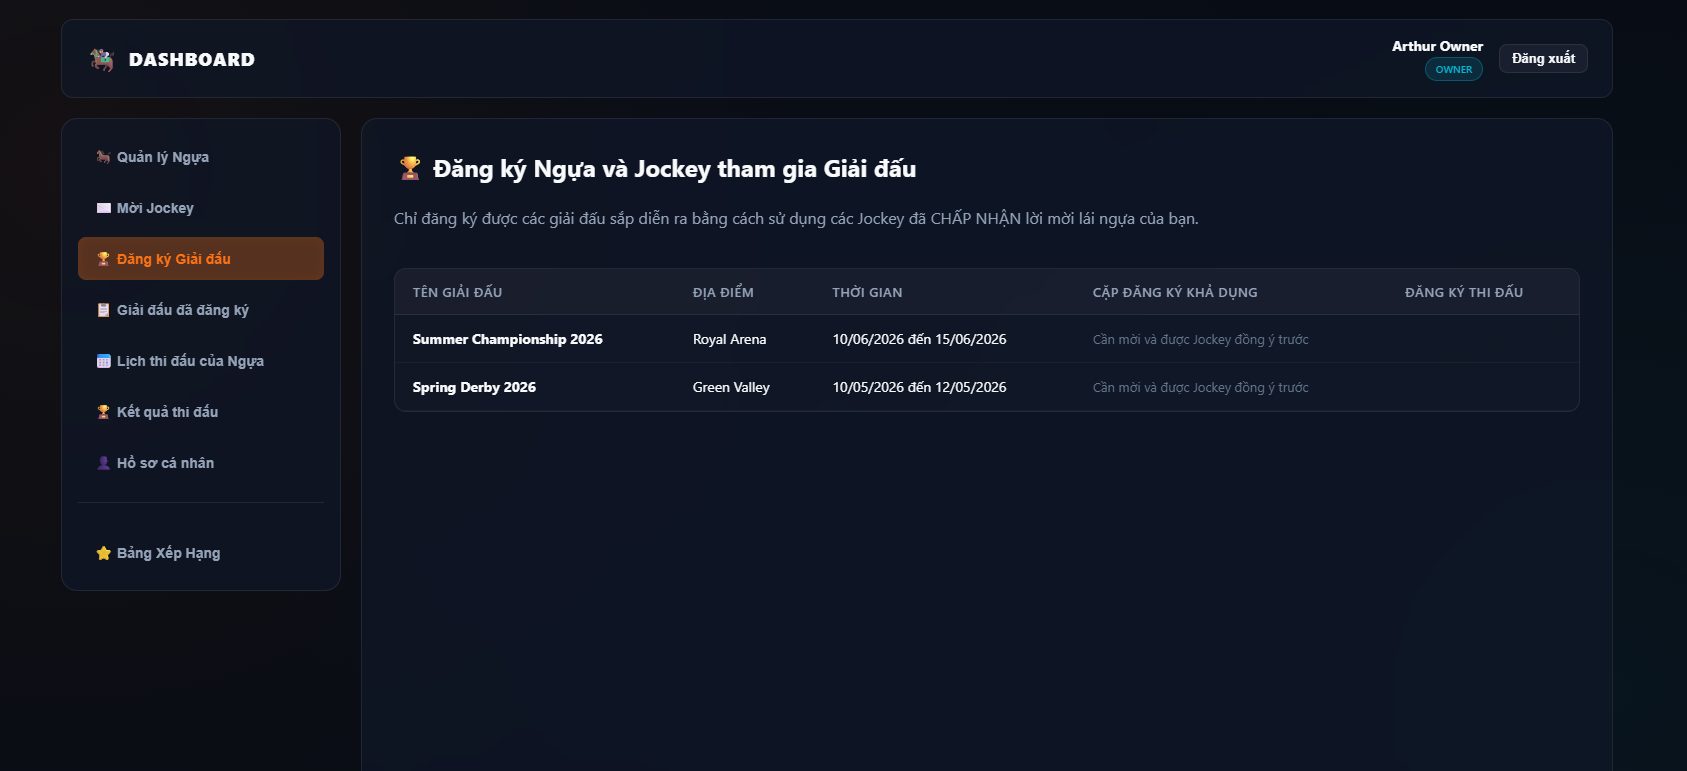
\includegraphics[width=\textwidth]{figures/web_application/owner/register_tournament.png}
    \caption{Tournament Registration}
\end{figure}

% ===================================================

\subsection{Registered Tournaments}

\textbf{Role:} Horse Owner

\begin{itemize}
    \item \textbf{Function trigger:} Select ``Giai dau da dang ky''.

    \item \textbf{Function description:}
    \begin{itemize}
        \item \textbf{Purpose:}
        \begin{enumerate}
            \item Monitor registration status.
            \item View approval results.
        \end{enumerate}

        \item \textbf{Data processing:}
        \begin{enumerate}
            \item Retrieve registration records.
            \item Retrieve approval status.
            \item Display registration history.
        \end{enumerate}
    \end{itemize}

    \item \textbf{Function details:}
    \begin{itemize}
        \item Display horse information.
        \item Display jockey information.
        \item Display approval status.
    \end{itemize}
\end{itemize}

\textbf{Screen layout:}

\begin{figure}[H]
    \centering
    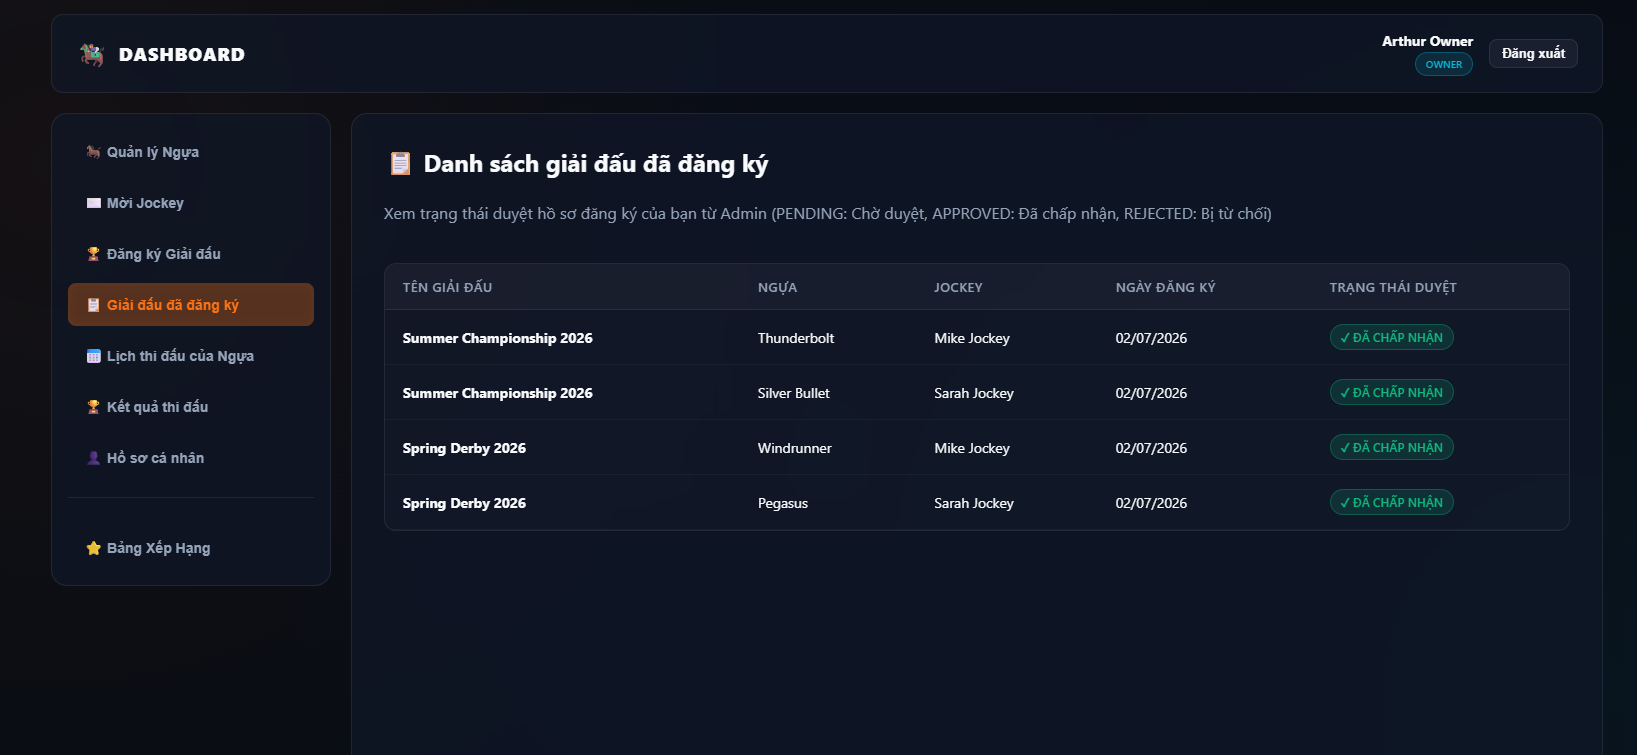
\includegraphics[width=\textwidth]{figures/web_application/owner/registered_tournament.png}
    \caption{Registered Tournaments}
\end{figure}

% ===================================================

\subsection{Horse Schedule}

\textbf{Role:} Horse Owner

\begin{itemize}
    \item \textbf{Function trigger:} Select ``Lich thi dau cua Ngua''.

    \item \textbf{Function description:}
    \begin{itemize}
        \item \textbf{Purpose:}
        \begin{enumerate}
            \item View upcoming races.
            \item Prepare for competitions.
        \end{enumerate}

        \item \textbf{Data processing:}
        \begin{enumerate}
            \item Retrieve race schedules.
            \item Retrieve tournament information.
            \item Display race information.
        \end{enumerate}
    \end{itemize}

    \item \textbf{Function details:}
    \begin{itemize}
        \item Display race date.
        \item Display location.
        \item Display tournament information.
    \end{itemize}
\end{itemize}

\textbf{Screen layout:}

\begin{figure}[H]
    \centering
    
\includegraphics[width=\textwidth]{figures/web_application/owner/schedule.png}
    \caption{Horse Schedule}
\end{figure}

% ===================================================

\subsection{Race Results}

\textbf{Role:} Horse Owner

\begin{itemize}
    \item \textbf{Function trigger:} Select ``Ket qua thi dau''.

    \item \textbf{Function description:}
    \begin{itemize}
        \item \textbf{Purpose:}
        \begin{enumerate}
            \item Review race results.
            \item Evaluate horse performance.
        \end{enumerate}

        \item \textbf{Data processing:}
        \begin{enumerate}
            \item Retrieve completed races.
            \item Retrieve rankings.
            \item Retrieve scores.
            \item Retrieve violations.
        \end{enumerate}
    \end{itemize}

    \item \textbf{Function details:}
    \begin{itemize}
        \item Display race rankings.
        \item Display accumulated points.
        \item Display remarks.
        \item Display violations.
    \end{itemize}
\end{itemize}

\textbf{Screen layout:}

\begin{figure}[H]
    \centering
    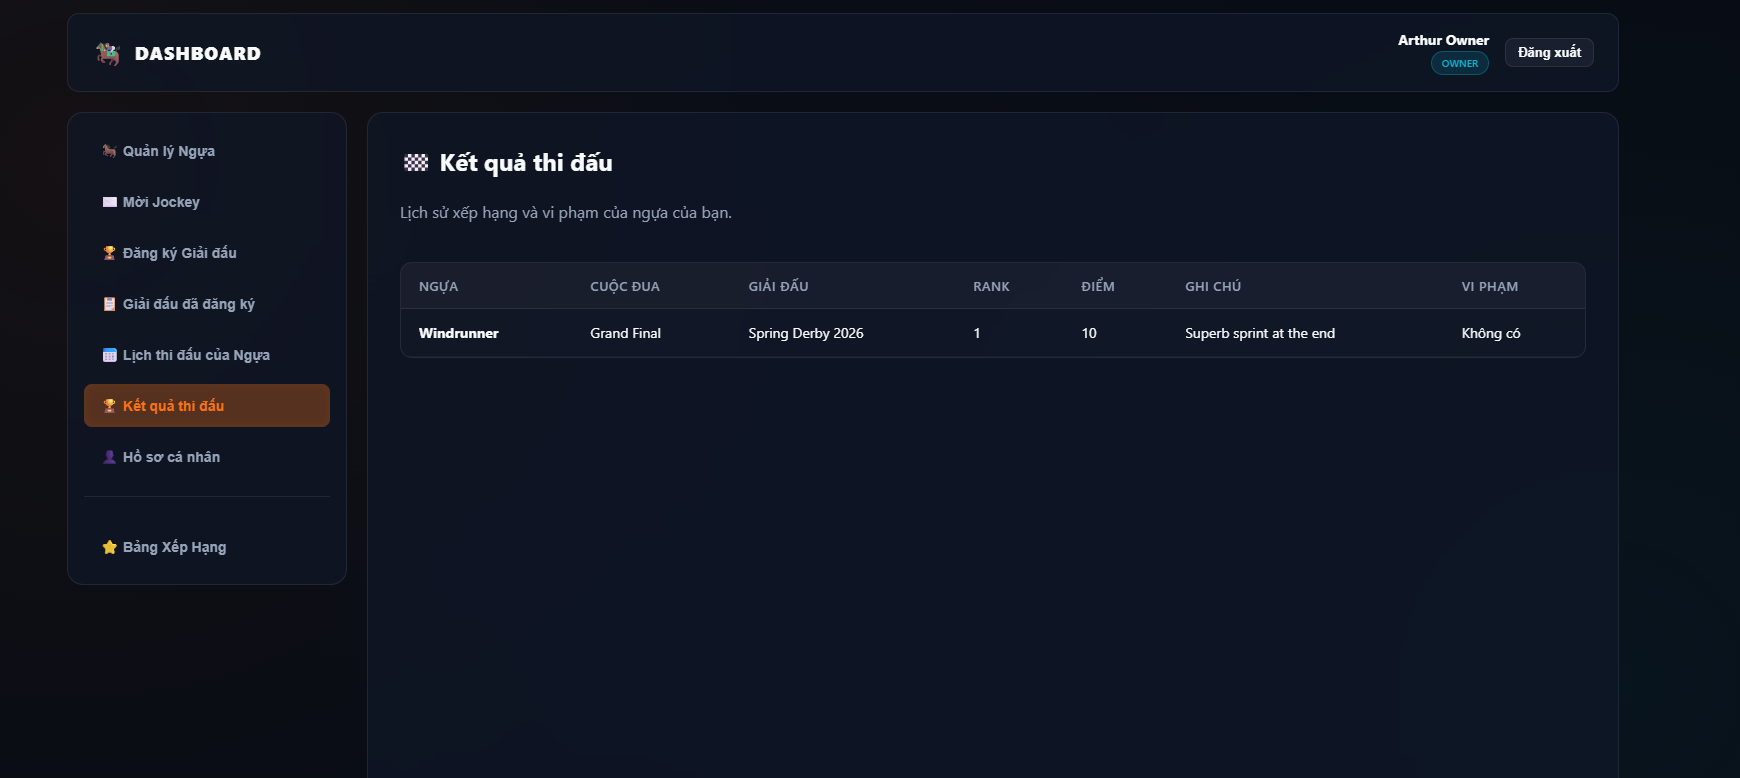
\includegraphics[width=\textwidth]{figures/web_application/owner/results.png}
    \caption{Race Results}
\end{figure}


\subsection{Owner Profile}

\textbf{Role:} Horse Owner

\begin{itemize}
    \item \textbf{Function trigger:} Select ``Ho so ca nhan''.

    \item \textbf{Function description:}
    \begin{itemize}
        \item \textbf{Purpose:}
        \begin{enumerate}
            \item Manage personal information.
            \item Update profile information.
        \end{enumerate}

        \item \textbf{Data processing:}
        \begin{enumerate}
            \item Update personal information.
            \item Update contact information.
            \item Update company information.
            \item Save profile data.
        \end{enumerate}
    \end{itemize}

    \item \textbf{Function details:}
    \begin{itemize}
        \item Edit owner profile.
        \item Edit biography.
        \item Update social information.
    \end{itemize}
\end{itemize}

\textbf{Screen layout:}

\begin{figure}[H]
    \centering
    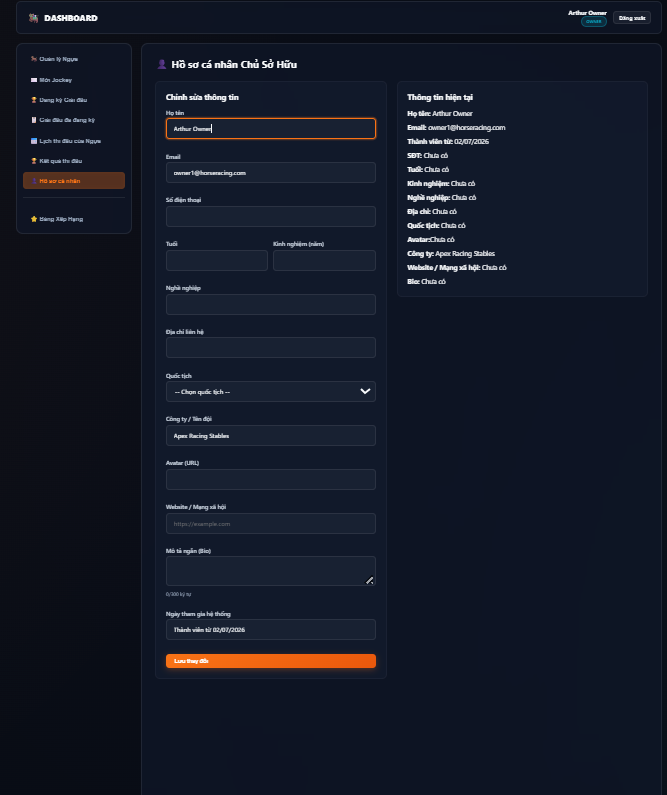
\includegraphics[width=0.9\textwidth]{figures/web_application/owner/profile.png}
    \caption{Owner Profile}
\end{figure}

% ===================================================

\subsection{Ranking}

\textbf{Role:} Horse Owner

\begin{itemize}
    \item \textbf{Function trigger:} Select ``Bang xep hang''.

    \item \textbf{Function description:}
    \begin{itemize}
        \item \textbf{Purpose:}
        \begin{enumerate}
            \item View official rankings.
            \item Compare competition performance.
        \end{enumerate}

        \item \textbf{Data processing:}
        \begin{enumerate}
            \item Retrieve horse rankings.
            \item Retrieve jockey rankings.
            \item Filter tournaments.
        \end{enumerate}
    \end{itemize}

    \item \textbf{Function details:}
    \begin{itemize}
        \item Display ranking positions.
        \item Display accumulated scores.
        \item Display tournament filters.
    \end{itemize}
\end{itemize}

\textbf{Screen layout:}

\begin{figure}[H]
    \centering
    
\includegraphics[width=\textwidth]{figures/web_application/owner/ranking.png}
    \caption{Ranking}
\end{figure}